\begin{question}
    Consider an aircraft with a canard, such that the aircraft has no tail, but has a control surface forward of the wings, as shown below. Assume the canard (shown in red) and the center of gravity are at the same vertical height relative to the zero lift line. You may also assume that $V=u_0$.

    \begin{figure}[h]
        \centering
        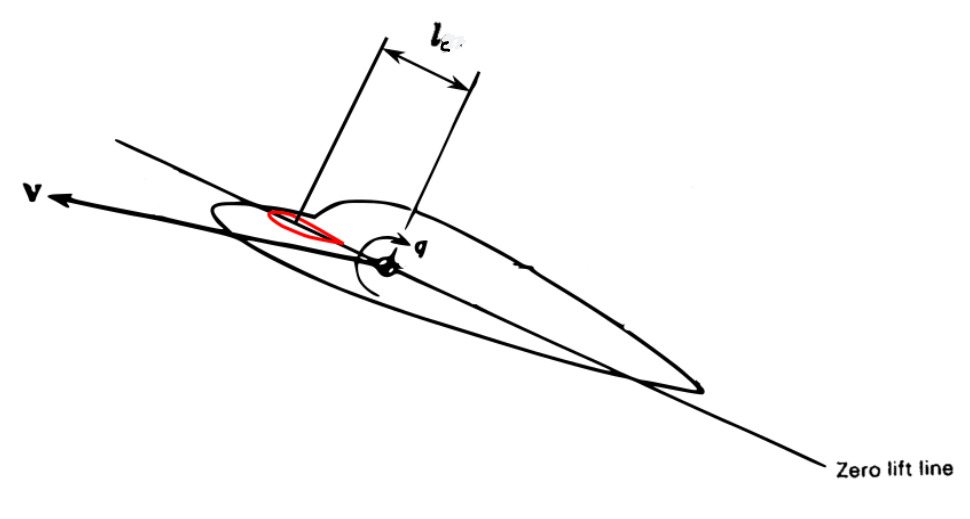
\includegraphics[width=0.5\textwidth]{questions/canard.png}
        % \caption{Caption}
        \label{fig:canard}
    \end{figure}

    The pitching moment coefficient for the canard $C_{m_c}$ is
    \begin{equation*}
        C_{m_c} = \frac{l_cS_c}{\bar{c}S}C_{l_c}=V_{H_c}C_{l_c},
    \end{equation*}
    where $S_c$ is the area of the canard, $S$ is the area of the wing, $l_c$ is the distance between the CG and the canard mean aerodynamic center, $\bar{c}$ is the length of the mean aerodynamic chord, and $V_{H_c}$ is the canard volume.

\begin{enumerate}
    \item Use a diagram to determine $\Delta \alpha_c$, the change in the effective angle of attack for the canard, as a function of $q$.
    \item Find $(C_{m_q})_{\text{canard}}$, the canard contribution to the pitching moment stability derivative.
\end{enumerate}

\end{question}
